\documentclass[11pt]{article}
\usepackage{amsmath}
\usepackage{amssymb}
\usepackage{amsthm} 
\usepackage{algorithm}
\usepackage{algpseudocode}
\usepackage{geometry}
\usepackage{fancyhdr}
\usepackage{tcolorbox}
\usepackage{titlesec}
\usepackage{booktabs}
\usepackage{hyperref}
\usepackage{tikz} 
\usetikzlibrary{arrows.meta,calc,positioning}
\usepackage{graphicx}   
\graphicspath{{./}{images/}}  

\usepackage{xcolor}

\newcommand{\ab}[1]{\textcolor{purple}{[#1 - AB]}}
\newcommand{\abedit}[1]{\textcolor{purple}{#1}}


\bibliographystyle{plain}
\renewcommand{\refname}{Bibliography}

% --- Theorem ---
\theoremstyle{plain}
% Define theorem environment
\newtheorem{theorem}{Theorem}
\renewcommand{\thetheorem}{2.\arabic{theorem}}

% page geometry
\geometry{a4paper, margin=1in}

% --- Header and Footer---
\pagestyle{fancy}
\fancyhf{}
\fancyhead[L]{\textbf{DS603}}
\fancyhead[C]{\textbf{Lecture 2 -- 01/08/2025}}
\fancyhead[R]{\textbf{Autumn 2025}}
\renewcommand{\headrulewidth}{0.4pt}
\fancyfoot[C]{2-\thepage}

\fancypagestyle{plain}{%
  \fancyhf{}%
  \renewcommand{\headrulewidth}{0pt}%
  \fancyfoot[C]{2-\thepage}%
}

\setcounter{secnumdepth}{3}

\titleformat{\subsection}
  {\Large\bfseries}
  {\thesubsection}
  {1em}
  {}

\titleformat{\subsubsection}[block]
  {\normalsize\bfseries}
  {\thesubsubsection}
  {1em}
  {}  

\renewcommand{\thesubsection}{2.\arabic{subsection}}
\renewcommand{\thesubsubsection}{2.\arabic{subsection}.\arabic{subsubsection}}



\begin{document}

\thispagestyle{plain}

\begin{tcolorbox}[colback=white, colframe=black, boxrule=1pt, sharp corners]
\textbf{DS603: Robust Machine Learning} \hfill \textbf{Autumn 2025}
\begin{center}
\vspace{2mm}
Lecture 2 -- 01/08/2025
\end{center}
\vspace{2mm}
\noindent\textit{Lecturer: Arjun Bhagoji \hfill Scribe: Akshaj Aithal, Rahul Kumar Yadav}
\end{tcolorbox}

\subsection{Efficient learning with convexity}

Since, we know that for the non-convex $0$-$1$ loss efficient learning is not possible, as its minimization is NP-hard(from Feldman et al 2012). Hence,
to enable tractable optimization, \textbfsurrogate losses} (e.g., hinge, logistic), are used, which can be minimized efficiently.
We know that, the surrogate loss needs to be \emph{classification-calibrated or consistent} with $0$-$1$ loss, as in that case, we can be sure that minimizing surrogate loss aligns with minimizing the $0$-$1$ risk.
Now, we need to ask under what conditions on the surrogate loss \& hypothesis class is
\textit{efficient learning} possible?


\subsubsection{Convexity}\label{sec:Convexity}
\begin{enumerate}
  \item $H$ must be a convex set $\Rightarrow \forall h, h',\alpha h + (1-\alpha)h' \in H$. 
  \item $l(h,z)$ must be a convex function in $h$ $\Rightarrow \forall z, l(\alpha h+(1-\alpha)h',z) \leq \alpha l(h,z) + (1-\alpha)l(h',z)$
\end{enumerate}

\small{Note: Implicitly treating $H\subset\mathbb{R}^d$ \& $h\in \mathbb{R}^d$}

\subsubsection{Boundedness}\label{sec:Boundedness}

Our hypothesis class $H$ needs to be bounded, which can be mathematically stated as $\forall h \in H$, $\lvert\lvert h \rvert\rvert_2 \leq B$, i,e. every element 
$h$ in the hypothesis class $H$ has bounded norm.


\subsubsection{Lipschitzness}\label{sec:Lipschitzness}
Let $l : \mathcal{Z} \times \mathcal{H} \to \mathbb{R}$ be a loss function, where $z \in \mathcal{Z}$ is a data point and $h \in \mathcal{H}$ is a hypothesis.  
We say that $l$ is \emph{$\rho$-Lipschitz in $h$, uniformly in $z$}, if  
\[
    |l(z,h) - l(z,h')| \leq \rho \, \|h - h'\|, 
    \quad \forall h,h' \in \mathcal{H}, \ \forall z \in \mathcal{Z}.
\]

In other words, for every data point $z$, $l(z,h)$ defines a loss curve that is Lipschitz continuous with the same constant $\rho$ for all $z$. 
The uniformity over $z$ ensures that the Lipschitz constant does not depend on the particular choice of $z$.

If $l(z,h)$ is differentiable in $h$, then the Lipschitz condition is \emph{equivalently} satisfied whenever
\[   
    \|\nabla_h l(z,h)\| \leq \rho, 
    \quad \forall h \in \mathcal{H}, \ \forall z \in \mathcal{Z}.
\]
\begin{itemize}
    \item The definition of Lipschitz continuity \emph{does not require differentiability}. 
          The gradient condition is only a sufficient characterization when $l$ is differentiable in $h$. 
    \item The gradient must be taken \emph{with respect to $h$}, not $z$, since Lipschitzness is being defined in terms of the hypothesis variable. 
    \item Bounded gradients guarantee Lipschitz continuity, but the converse is not always true: 
          a function can be Lipschitz continuous without being differentiable everywhere (e.g., the hinge loss). 
\end{itemize}


\subsubsection{Smoothness}\label{sec:Smoothness}
We say a function $l$ to be smooth if,
\[
\forall z,h,h' \lvert\lvert \nabla l(z,h) - \nabla l(z,h')\rvert\rvert \leq \beta\lvert\lvert h-h'\rvert\rvert 
\]
\[
\text{where } \{z,h\} \text{ and } \{z, h'\} \in \text{the domain of function }l, \text{and } \beta \text{ is some constant}.
\]

% refine paragraph below
With convex sets that satisfy ~\ref{sec:Convexity}, ~\ref{sec:Boundedness} \& ~\ref{sec:Lipschitzness}, or  ~\ref{sec:Convexity}, ~\ref{sec:Boundedness} \& ~\ref{sec:Smoothness} we get problems that are learnable and usually efficient.

\noindent \textbf{Note}: There exist convex learning problems that satisfy
~\ref{sec:Convexity}, ~\ref{sec:Boundedness} \& ~\ref{sec:Lipschitzness} that
are not efficiently learnable. See 12.6.4 in \cite{ShalevShwartzUnderstandingML}.

\subsection{Optimizing over Vector Spaces}
Let $\vec{\theta}\in\mathbb{R}^d$ and let $f:H\to\mathbb{R}$. We want to minimize $f(\vec{\theta})$ over
\[
  H \;=\; \bigl\{\vec{\theta}\in\mathbb{R}^d : \lVert \vec{\theta}\rVert_2 \le B \bigr\}.
\]
Additionally, assume that $f$ is convex and $L$-Lipschitz; for simplicity, also assume that $f$ is differentiable.

\smallskip
\noindent\textit{Note:} Convex functions always admit subgradients but need not be differentiable everywhere. We gloss over this for simplicity.


\subsubsection{Subgradient Lemma}
\textbf{Lemma:}  
Let $H \subseteq \mathbb{R}^d$ be a convex set and $f : H \to \mathbb{R}$ be a convex function.  
Then, for any $\vec{\theta}_1, \vec{\theta}_2 \in H$ and any subgradient $g \in \partial f(\vec{\theta}_2)$, we have
\[
    f(\vec{\theta}_1) - f(\vec{\theta}_2) \;\ge\; g^\top \big(\vec{\theta}_1 - \vec{\theta}_2\big).
\]

\begin{itemize}
    \item $\vec{\theta}_1, \vec{\theta}_2 \in H$ are two points in the domain of $f$.
    \item $f : H \to \mathbb{R}$ is a convex function.
    \item $g \in \partial f(\vec{\theta}_2)$ is a subgradient of $f$ at $\vec{\theta}_2$ (i.e., $g$ satisfies the subgradient inequality above).
\end{itemize}

If $f$ is differentiable at $\vec{\theta}_2$, then the subdifferential $\partial f(\vec{\theta}_2)$ is the singleton $\{\nabla f(\vec{\theta}_2)\}$, and the lemma becomes:
\[
    f(\vec{\theta}_1) - f(\vec{\theta}_2) \;\ge\; \nabla f(\vec{\theta}_2)^\top \big(\vec{\theta}_1 - \vec{\theta}_2\big).
\]


The key question arises is how do we optimize a convex-bounded Lipschitz function?

\subsubsection{Projection Lemma}


\begin{figure}[h]
\centering
\begin{tikzpicture}[scale=2.0, every node/.style={scale=1}]
  %---- switch here if you want Π_H(x) instead of Π_H(ω)
  \def\projarg{\omega}

  % Coordinates
  \coordinate (omega) at (0,2);
  \coordinate (theta) at (1.05,-0.35);
  \coordinate (center) at (0,0);
  \def\r{2}
  % Choose a projection point on the boundary (on the circle)
  \coordinate (proj) at (1.8,1.5); % on circle arc

  % Convex set (ball boundary; draw only an arc to match the look)
  \draw[line width=0.6pt] ($(center)+(3, -0.35)$) arc[start angle=0,end angle=180,radius=\r];

  % Points
  \fill (omega) circle (0.02) node[above left=2pt] {$\omega$};
  \fill (theta) circle (0.02) node[below right=2pt] {$\theta$};
  \fill (proj)  circle (0.02) node[above right=2pt] {$\Pi_H(\projarg)$};

  % Main segment ω--θ
  \draw[line width=0.6pt] (omega) -- (theta);

  % Dotted segments: b = ω--proj, a = θ--proj
  \draw[dotted, line width=0.8pt] (omega) -- (proj);
  \draw[dotted, line width=0.8pt] (theta) -- (proj);

  % Labels a and b near the dotted segments
  \node[blue] at ($ (omega)!0.55!(proj) + (0.02,0.02) $) {\small b};
  \node[blue] at ($ (theta)!0.55!(proj) + (0.10,0.00) $) {\small a};
\end{tikzpicture}
\caption{Projection Lemma}
\end{figure}

Let $H \subseteq \mathbb{R}^d$ be a nonempty, closed, convex set, and let
\[
\Pi_H(x) := \arg\min_{y \in H} \|x-y\|_2
\]
denote the Euclidean projection of $x$ onto $H$. Then, for any $\omega \in \mathbb{R}^d$ 
and any $\theta \in H$, we have
\[
    \|\theta - \Pi_H(\omega)\|_2^2 \;+\; \|\omega - \Pi_H(\omega)\|_2^2 
    \;\leq\; \|\omega - \theta\|_2^2.
\]
, which for our figure becomes

\[
\lvert\lvert\vec{a}\rvert\rvert^2 + \lvert\lvert\vec{b}\rvert\rvert^2 \leq \lvert\lvert \omega -\theta\rvert\rvert^2
\]

This inequality expresses the Pythagorean property of Euclidean projection: the projection 
point $\Pi_H(\omega)$ is the closest point in $H$ to $\omega$.

\subsubsection{Projected Gradient Descent}
Projected Gradient Descent (PGD) is an iterative optimization method for constrained problems of the form 
\[
    \min_{\vec{\theta} \in H} f(\vec{\theta}),
\]
where $H \subseteq \mathbb{R}^d$ is a convex feasible set.  
Starting from an initial point $\vec{\theta}_0 \in H$, the update rule is
\[
    \vec{\omega}_{t+1} = \vec{\theta}_t - \eta \, \nabla f(\vec{\theta}_t),
\]
\[
    \vec{\theta}_{t+1} = \Pi_H\big(\vec{\omega}_{t+1}\big),
\]
where $\eta > 0$ is the step size and $\Pi_H(\cdot)$ denotes the Euclidean projection onto $H$, defined as
\[
    \Pi_H(\vec{x}) = \arg\min_{\vec{y} \in H} \; \lVert \vec{y} - \vec{x} \rVert_2.
\]
The projection step ensures that $\vec{\theta}_{t+1}$ remains in $H$ by projecting any infeasible point $\vec{\omega}_{t+1} \notin H$ back to the closest point in $H$ in terms of Euclidean distance.

\begin{theorem}
Using $\eta = \frac{B}{\rho \sqrt{T}}$, where $\rho$ is the Lipschitz constant of $f$ and $\vec{\theta}^*$ its minimizer in $H$, we have
\[
    f\!\left( \frac{1}{T} \sum_{t=1}^T \vec{\theta}_t \right) - f(\vec{\theta}^*) \;\le\; \frac{B\rho}{\sqrt{T}}.
\]
\end{theorem}

\begin{proof}
\textbf{Subgradient lemma at $\theta_t$.}
By convexity (subgradient inequality with $g_t=\nabla f(\theta_t)\in\partial f(\theta_t)$),
\[
f(\theta_t)-f(\theta^*) \;\le\; g_t^{\top}(\theta_t-\theta^*).
\]

\textbf{Three-point identity.}
Using the elementary identity
\[
2a^{\top}b=\|a\|_2^2+\|b\|_2^2-\|a-b\|_2^2
\]
with $a=\theta_t-\theta^*$ and $b=\theta_t-\omega_{t+1}=\eta g_t$, we get
\[
g_t^{\top}(\theta_t-\theta^*)
=\frac{1}{2\eta}\!\left(\|\theta_t-\theta^*\|_2^2-\|\omega_{t+1}-\theta^*\|_2^2\right)
+\frac{\eta}{2}\,\|g_t\|_2^2.
\]

\textbf{Nonexpansiveness of projection.}
Since Euclidean projection is nonexpansive and $\theta^*\in H$,
\(
\|\omega_{t+1}-\theta^*\|_2 \ge \|\theta_{t+1}-\theta^*\|_2.
\)
Hence
\[
f(\theta_t)-f(\theta^*) \;\le\;
\frac{1}{2\eta}\!\left(\|\theta_t-\theta^*\|_2^2-\|\theta_{t+1}-\theta^*\|_2^2\right)
+\frac{\eta}{2}\,\|g_t\|_2^2.
\]

\textbf{Sum and telescope.}

Summing $t=1$ to $T$, applying the telescoping identity 

\[
\sum_{t=1}^T \bigl(\|\theta_t-\theta^*\|_2^2 - \|\theta_{t+1}-\theta^*\|_2^2\bigr) 
= \|\theta_1-\theta^*\|_2^2 - \|\theta_{T+1}-\theta^*\|_2^2,
\] 
and using $\|g_t\|_2 \le \rho$ together with the fact that 
$-\|\theta_{T+1}-\theta^*\|_2^2 \le 0$, thus, $\|\theta_1-\theta^*\|_2^2 - \|\theta_{T+1}-\theta^*\|_2^2$ $\le$ $\|\theta_1-\theta^*\|_2^2$, we obtain
\[
\sum_{t=1}^T \bigl(f(\theta_t)-f(\theta^*)\bigr)
\;\le\; \frac{\|\theta_1-\theta^*\|_2^2}{2\eta} \;+\; \frac{\eta\rho^2 T}{2}.
\]


\textbf{Average and choose $\eta$.}
By convexity of $f$,
\(
f\!\left(\frac1T\sum_{t=1}^T\theta_t\right)\le \frac1T\sum_{t=1}^T f(\theta_t).
\)
Divide the previous inequality by $T$ and take
\(\eta=\frac{B}{\rho\sqrt{T}}\):
\[
f\!\left(\frac1T\sum_{t=1}^T\theta_t\right)-f(\theta^*)
\;\le\; \frac{B^2}{2\eta T}+\frac{\eta\rho^2}{2}
\;=\; \frac{B\rho}{2\sqrt{T}}+\frac{B\rho}{2\sqrt{T}}
\;=\; \frac{B\rho}{\sqrt{T}}.
\]
\end{proof}

\textbf{Note}:The rate is dimension independent!

The key question which now arises is how we can use gradient descent for learning?

\subsection{Learning with Gradient Descent}

\underline{Option 1}:
\[
f(\vec{\theta}) = \frac{1}{n} \sum_{i=1}^{n} l(\vec{z}_i, \vec{\theta}) = \hat{L}(\vec{\theta})
\]
\\
\underline{Option 2}:
\[
f(\vec{\theta}) = \mathbb{E}_{\vec{z} \sim p^*} \left[ l(\vec{z}, \vec{\theta}) \right] = L(\vec{\theta})
\]\\

In Option 2, we do not have access to the full distribution, so we use (fresh) random samples.

\subsubsection{Stochastic Gradient Descent}
In SGD, we don't do gradient descent over all of the dataset, rather we use only

some datapoints for the process of updation. Typically, when the number of datapoints, $z^* =1$, then it is termed as Stochastic Gradient Descent, else it is called mini-batch gradient descent. When batch size equals $1$, then  For $t = 1, \dots, T$, sample $\vec{z}_t \sim p^*$.  

Then,
\[
\vec{\omega}_{t+1} = \vec{\theta}_t - \eta \, \nabla_\theta l(\vec{z}_t, \vec{\theta}_t),
\]
\[
\vec{\theta}_{t+1} = \Pi_H(\vec{\omega}_{t+1}).
\]

Similarly, in the case of mini-batched gradient descent to update, we take average of gradient over all the data points sampled equaling the batch size for that time $t$,
At iteration $t$, sample a mini-batch $B_t$ of size $m$.  
The update rule is given by

\[
\theta_{t+1} 
= \theta_t - \eta \cdot \frac{1}{m} \sum_{i \in B_t} \nabla_\theta \, l(z_i, \theta_t),
\]
We can apply projection rule as above, if needed.
\begin{theorem}
If $\eta = \frac{B}{\rho \sqrt{T}}$, then
\[
\mathbb{E}_{\{\vec{z}_t\}_{t=1}^T} \left[ L\!\left( \frac{1}{T} \sum_{t=1}^T \vec{\theta}_t \right) \right]
- L(\vec{\theta}^*)
\;\le\; \frac{B\rho}{\sqrt{T}}.
\]
\end{theorem}

\noindent\textbf{Note:} This is effectively a new learning paradigm, but it needs fresh samples at each step.  
Otherwise, the underlying assumption that the stochastic gradient is an unbiased estimator of the loss does not hold.

\medskip
\noindent 
In Option 1, we can make as many passes over the data as we wish. \textit{(Why is this true?)} 

\subsection{Vacuous Bounds in Statistical Learning Theory}

In classical Statistical Learning Theory (SLT), the \textit{fundamental theorem of statistical learning} states that to guarantee generalization within error $\varepsilon$ with high probability, it suffices to have
\[
m \;\gtrsim\; \frac{\log |\mathcal{H}|}{\varepsilon^2},
\]
where $m$ is the number of training samples and $\mathcal{H}$ is the hypothesis class.

\subsubsection*{A High-Dimensional Example}
Let $\vec{\theta} \in \mathbb{R}^d$, and assume each coordinate is represented with $32$ bits. Then the number of possible parameter configurations is
\[
|\mathcal{H}| = \left( 2^{32} \right)^{d}.
\]
Taking logarithms,
\[
\log |\mathcal{H}| = 32\,d.
\]
The sample complexity bound becomes
\[
m \;\gtrsim\; \frac{32\,d}{\varepsilon^2}.
\]
For large $d$ (as in modern deep networks), this bound predicts an astronomically large $m$, often much larger than what is available in practice.

\subsubsection*{Why the Bound is Vacuous}
In modern machine learning the number of training samples needed to get low test error is much smaller than that predicted by the fundamental theorem of statistical learning, thus, the bound on number of samples is of not much help to us! Thus, we need new theoretical approaches to understand how learning happens in the case of neural networks.

\subsubsection{Double Descent}

\begin{figure}[ht]
  \centering
  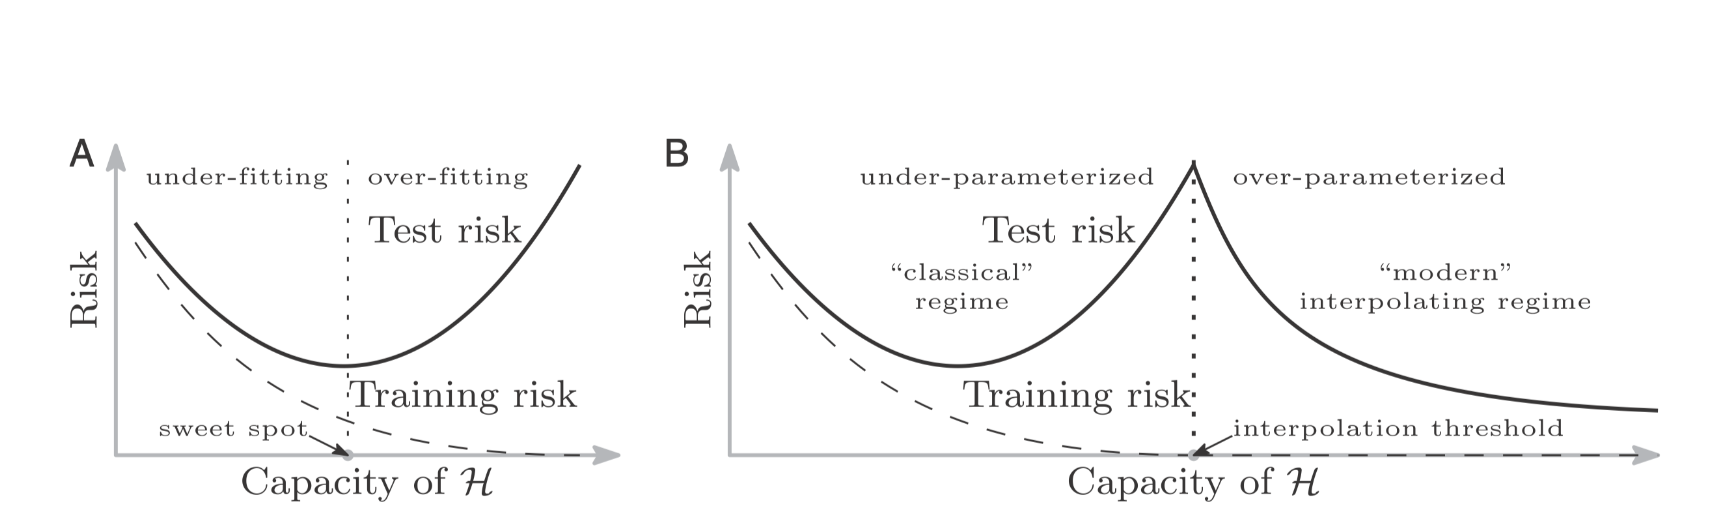
\includegraphics[width=\linewidth]{DoubleDescent.png}
  \caption{Double descent: test risk (solid) and training risk (dashed) as model capacity increases.}
  \label{fig:double-descent}
\end{figure}

The \textit{double descent} phenomenon describes a relationship between model complexity and generalization error. 
In the classical case, there is something called as bias--variance tradeoff in which test error decreases as complexity of the model increases until it reaches an optimal point, after which it starts to increase due to overfitting.
However, a newer kind of phenomenon in modern overparameterized models (e.g., deep neural networks) is observed, in which, increasing complexity beyond the interpolation threshold, where the model fits the training data exactly can lead to a second regime where test error decreases again. 


\subsection{Unsupervised Learning \& Anomaly Detection}


Much of the material in this section is adapted from the survey namely \emph{A Unifying Review of Deep and Shallow Anomaly Detection by Lukas Ruff et al.}, which provides a comprehensive review of deep and shallow anomaly detection methods.

\subsubsection{Assumptions in Traditional Supervised Learning}
\begin{enumerate}
  \item \textbf{Labeled data available:} training examples $(x_i,y_i)$ are provided.
  \item \textbf{Train--test i.i.d.:} both sets are drawn from the same distribution
  \[
    (x,y)\sim P_{\text{train}}=P_{\text{test}}.
  \]
  \textit{Remark:} When the second assumption fails, we study distributionally
  robust optimization and domain adaptation to handle covariate shift, concept
  drift, label shift, etc..
\end{enumerate}

\subsubsection{Unsupervised Learning}
We observe unlabeled samples
\[
  \{x_i\}_{i=1}^n \stackrel{\text{i.i.d.}}{\sim} P^{+}\ \text{on}\ \mathcal X,
\]
and no labels are provided.

\subsubsection{Anomaly Detection}
\paragraph{Basic problem:}
Given a new point $\tilde x$, decide whether it is \emph{in-distribution} (i.e., typical of $P^{+}$).
If $P^{+}$ has a probability density function, then we chose a threshold $\tau\ge 0$ and define the anomaly set as
\[
  \mathcal A := \{x\in\mathcal X \;:\; p^{+}(x)\le \tau\}.
\]

\paragraph{Challenges:}
\begin{enumerate}
  \item Modeling $P^{+}$ is hard. Misspecification leads to errors:
  \[
    \text{FPR}=\Pr_{x\sim P^{+}}[\hat y(x)=\text{anomaly}],\quad
    \text{FNR}=\Pr_{x\sim P^{\text{anom}}}[\hat y(x)=\text{normal}].
  \]
  High complexity of $P^{+}$ can cause either large FPR (typical $x\sim P^{+}$ wrongly flagged) or large FNR (true anomalies missed).
  \item Anomalies may come from arbitrary, heterogeneous distributions $\{P^{i}\}$ (one or many) and are rare.
\end{enumerate}

\paragraph{Model of Normality:}
Since we have samples from $P^{
+
}$, we try to model \emph{normality} directly and treat all training examples as label $1$ (normal).

\subsubsection{Notes on terminology and assumptions}
The terms \emph{anomaly}, \emph{novelty}, and \emph{outlier} are used differently across fields:
\begin{itemize}
  \item \textbf{Anomaly:} out-of-support/semantically different (e.g., a \emph{dog} when $P^{+}$ is cats).
  \item \textbf{Outlier:} a rare/extreme point from $P^{+}$ (e.g., a rare breed of cat far in the tail).
  \item \textbf{Novelty:} previously unseen but related subpopulation.(e.g., a new cat breed).
\end{itemize}

\paragraph{Contamination}
\begin{enumerate}
  \item \textbf{Question.} How do we know all observed examples truly come from $P^{+}$? What if there is noise or corruption?
  \item \textbf{More general model (Huber $\varepsilon$-contamination).}
  \[
    x_i \sim (1-\varepsilon)\,P^{+} \;+\; \varepsilon\,Q\;+\;noise,\qquad 0\le \varepsilon<1,
  \]
  where $Q$ is an arbitrary (adversarial or unknown) distribution.
\end{enumerate}

\paragraph{Other Unsupervised Learning Methods}
Below are some methods which we can use to look for the anomalies:-
\begin{enumerate}
  \item \textbf{Clustering:} k-means.
  \item \textbf{Reconstruction-based:} PCA, Autoencoders.
\end{enumerate}



\begin{thebibliography}{99}

\bibitem{ShalevShwartzUnderstandingML}
Shai Shalev-Shwartz and Shai Ben-David.
\newblock \emph{Understanding Machine Learning: From Theory to Algorithms}.
\newblock Cambridge University Press, 2014.

\bibitem{LiangStatsLearnNotes}
Percy Liang.
\newblock \emph{Statistical Learning Theory Notes}.
\newblock Stanford University, 2023.
\newblock Available at \url{https://web.stanford.edu/~pliang/cs229/}.

\bibitem{Salehi, M., Mirzaei, H., Hendrycks, D., Li, Y., Rohban, M. H., & Sabokrou, M. (2021). A Unified Survey on Anomaly, Novelty, Open-Set, and Out-of-Distribution Detection: Solutions and Future Challenges.}
\newblock \emph{Salehi, M., Mirzaei, H., Hendrycks, D., Li, Y., Rohban, M. H., and Sabokrou, M. (2021). A Unified Survey on Anomaly, Novelty, Open-Set, and Out-of-Distribution Detection: Solutions and Future Challenges.}
\newblock ArXiv. \url{https://arxiv.org/abs/2110.14051}

\bibitem{Convex Optimization: Algorithms and Complexity — Sébastien Bubeck (2015 lecture notes)}
\newblock \emph{Convex Optimization: Algorithms and Complexity — Sébastien Bubeck (2015 lecture notes)}

\bibitem{A Unifying Review of Deep and Shallow Anomaly Detection}
\newblock \emph{A Unifying Review of Deep and Shallow Anomaly Detection. \url{https://arxiv.org/abs/2009.11732}}


\end{thebibliography}

\end{document}